\section{Experimental Setup}
\label{expSetup}

%%%%%%%%%%%%%%%%%%%%%%%%%%%%%%%%%%%%%%%%%%%%%%%%%%%%%%%%%%%%%%%%%%%%%%%%%%%%%%%%%%%%%%%%%%%%%%%%%%%%%%%%%%%%%%%
%Initiator: Ran Itay
%Last modified by: MM Devi, May 26 2017
%Comment: The detector section has been modified. MMdevi's changes are made in blue
%%%%%%%%%%%%%%%%%%%%%%%%%%%%%%%%%%%%%%%%%%%%%%%%%%%%%%%%%%%%%%%%%%%%%%%%%%%%%%%%%%%%%%%%%%%%%%%%%%%%%%%%%%%%%%%

In order to identify superradiance effects in LXe, the temporal and spatial properties of a scintillation event should be studied and quantified. In the DIREXENO system LXe is circulated through a small spherical cavity held in a thick high purified fused silica (HPFS) sphere . The sphere is surrounded (4$\pi$) by PMTs allowing a high resolution spatial and temporal measurements of individual photons. The PMTs and wires do not come in contact with the xenon, so less impurities are introduced to it, and the material selection is less stringent. The geometrical design of the system simulates a point like source of scintillation photons, and a detailed vertex reconstruction within the LXe drop is unnecessary. A schematic view of the system is shown in Fig~\ref{fig:detSch} . 

\begin{figure}[h]
\centerline{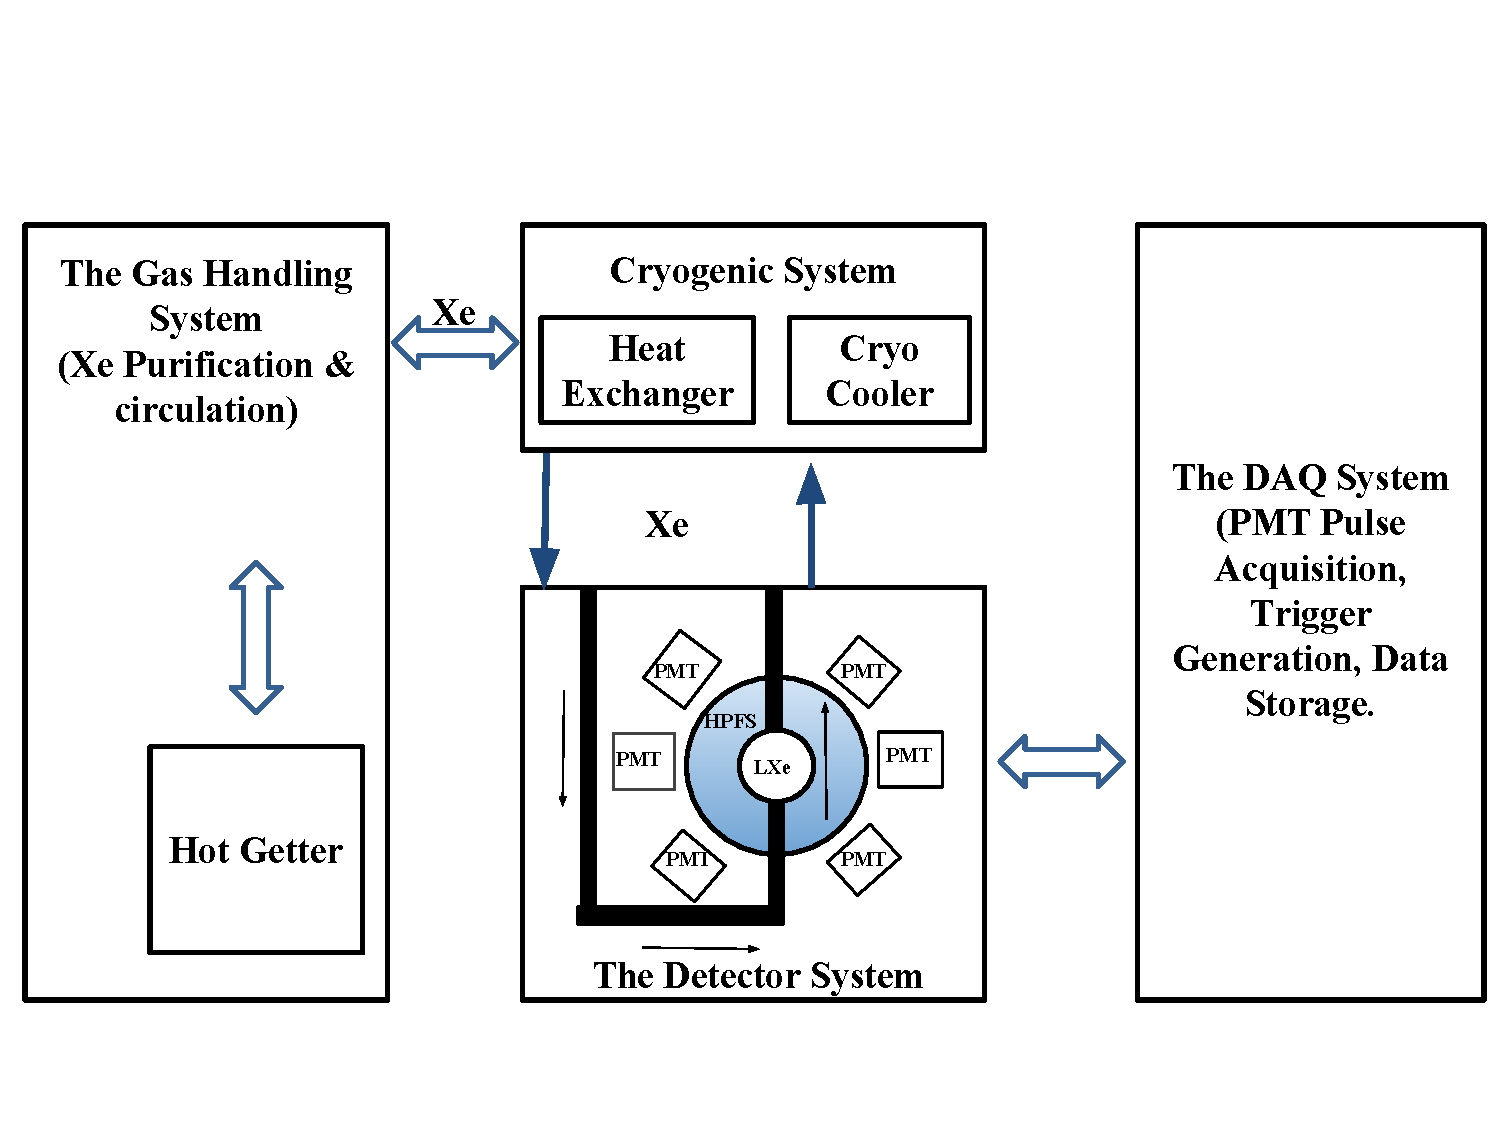
\includegraphics[width=0.8\linewidth]{DetSch.pdf}}
\caption{A schematic view of DIREXENO.}
\label{fig:detSch}
\end{figure}


The current system is designed with \RanComment{TODO check digitzation time} $\sim1$\,ns time resolution, $<1$\,ns synchronization between PMTs, and XX radians spatial resolution. Since the exact nature and magnitude of superradiance in LXe is yet unknown a guiding principle in the design was flexibility to upgrades or redesign of any part of the system to fulfill any future experiment requirements. In addition we gain fast and easy recovery in case of components malfunction. This is achieved by a modular design. 

Four main building blocks constitute the system. (i) \textbf{The gas handling system} which in normal working mode circulates the xenon through the setup and  purifies it. (ii) \textbf{The cryogenic system}, liquefies the xenon and 
delivers it to the detector system. (iii) \textbf{The detector system} consists of a fused silica sphere that 
holds a small bubble of LXe target, and PMTs around the sphere. (iv) \textbf{The DAQ system} supplies high voltage (HV) 
to the PMTs and the handles monitoring, triggering and digitization. The entire assembly is held on 3 separate racks as shown in Fig.~\ref{fig:fulldet}.
 

%The experimental setup of DIREXENO is described in this section. This setup is  designed to measure the spatial and temporal properties of LXe scintillation. It consists of a modular design in order to extend its flexibility to fulfill the requirement of any different future experiments. 

%The four main building blocks constitutes of the full setup, a schematics 
%of which, with the interfaces between them is shown in Fig.~\ref{fig:fullschematics}. 
%The gas handling system, in normal working mode, drives the xenon from the detector through 
%a purifier and cycles it back into the detector. The cryogenic system, liquefies the xenon and 
%delivers it to the detector system. The detector system consists of a fused silica sphere that 
%holds a small bubble of LXe target, and PMTs around the sphere. The supply of high voltage (HV) 
%to the PMTs and the data readout are carried out through the 
%data acquisition system (DAQ) system. 
%These four building blocks are independent of each other construction wise, and can be 
%replaced without altering features in the others. 

%\begin{figure}[h]
%\centerline{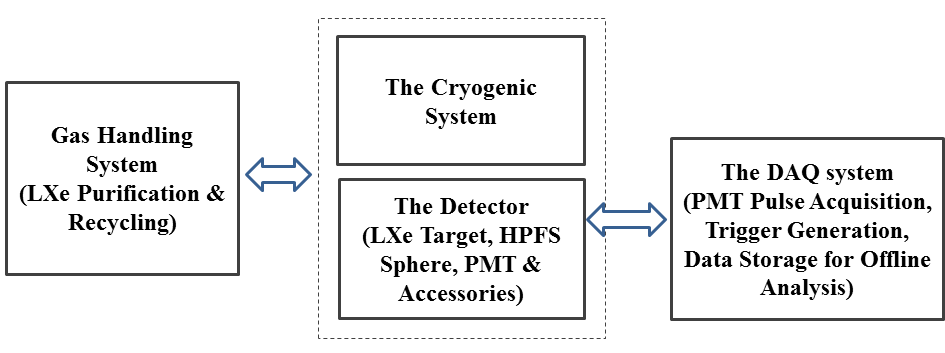
\includegraphics[width=0.8\linewidth]{WholeSys.png}}
%\caption{A schematic of DIREXENO showing all the four building blocks of the system.}
%\label{fig:fullschematics}
%\end{figure}



\begin{figure}[h]
\centerline{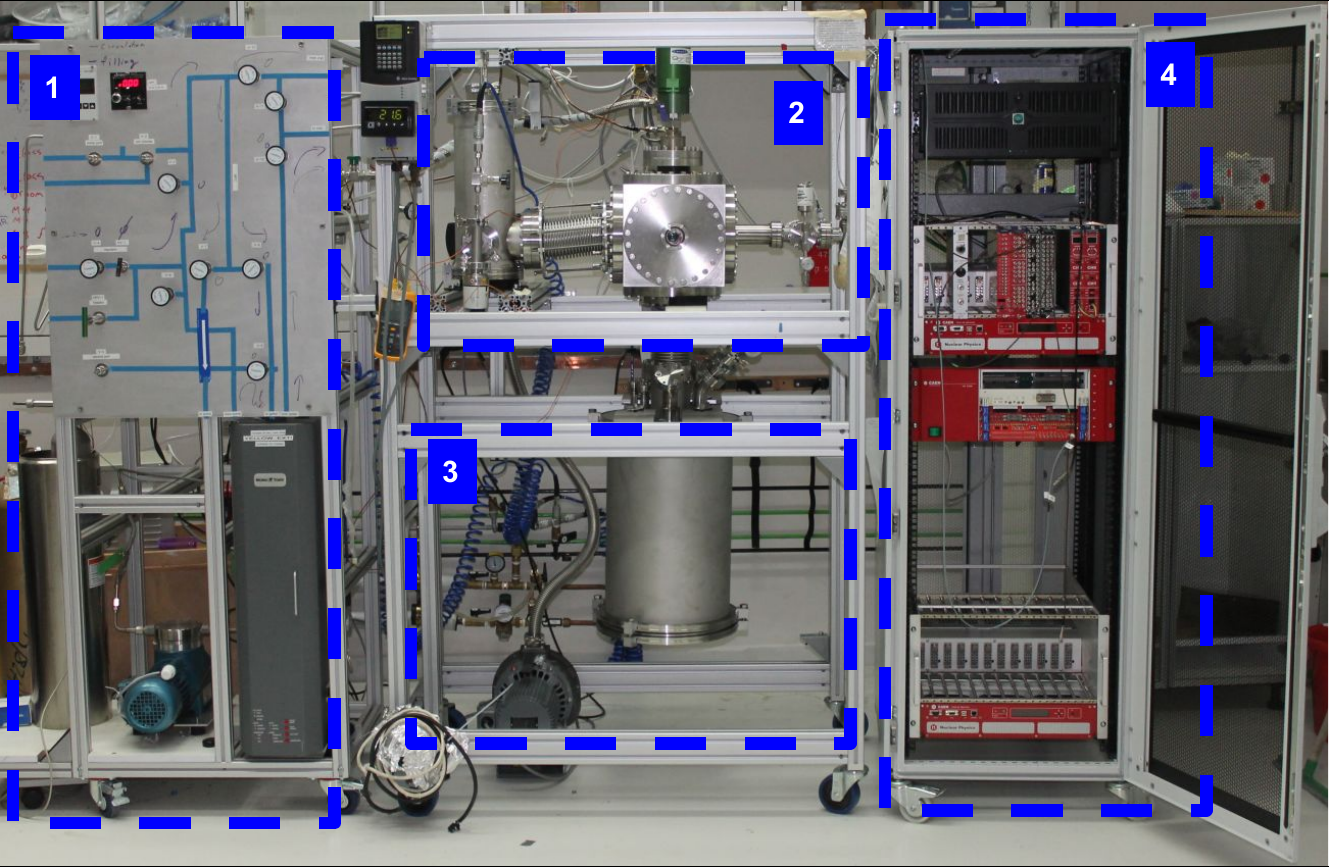
\includegraphics[width=0.8\linewidth]{FullSys.png}}
\caption{DIREXENO. 1. The gas handling system. 2. The cryogenic system including the heat exchanger. 3. The detector chamber. 4. The Data acquisition system.}
\label{fig:fulldet}
\end{figure}



\subsection{The gas handling system}
\label{subsec:gas}

In DIREXENO only the prompt scintillation is measured, therefore a high level of purity is not of a great importance. However in many LXE detectors the desired level of impurity concentration is at the level of 1 ppb $O_2$ equivalent~\cite{Aprile:2009dv}
%While in DIREXENO a high level of purity is not of a great importance as only the prompt scintillation is measured, in many LXE detectors the desired level of impurity concentration is at 
%the level of 1 ppb $O_2$ equivalent~\cite{Aprile:2009dv}. 
This is crucial to allow 
ionization electrons drift for several cm. To reach that level in a reasonable amount 
of time (several days instead of months), 
a continuous purification is needed. The gas handling system provides this process along 
with all gas handling operations such as filling and recuperation. The xenon circulation also plays a major role in heat transfer, as will be discussed in ~\ref{subsec:det}.


During purification, The xenon is forced by a circulation pump\footnote{N143 SN.12E AC 230V50HZ KNF diaphragm circulation pump} extracting LXe from the detector part through a heat exchanger\footnote{GEA GBS100M-24 plate heat exchanger} 
where it is heated and vaporized, into a hot getter\footnote{MONO-TORR PS4-MT15-R-2} which cleans the xenon. The xenon passes through a mass flow controller\footnote{MKS mass flow controller} (MFC), 
enabling monitoring and controlling the amount of heat introduced to the system.  Once purified, the xenon is delivered back to the cryogenic system 
via the heat exchanger, where the remaining GXe is 
liquefied before it continues back to the detector part. A schematic of this 
system is shown in fig.~\ref{fig:gasSchematic}.


%%%%%%%%%%%%%%%%%%%%%%%%%%%%%%%%%%%%%%%%%%%%%%%%%%%%%%%%%%%%%%%%%%%%%%%%%%%%%%%%%%
\begin{figure}[h]
\centerline{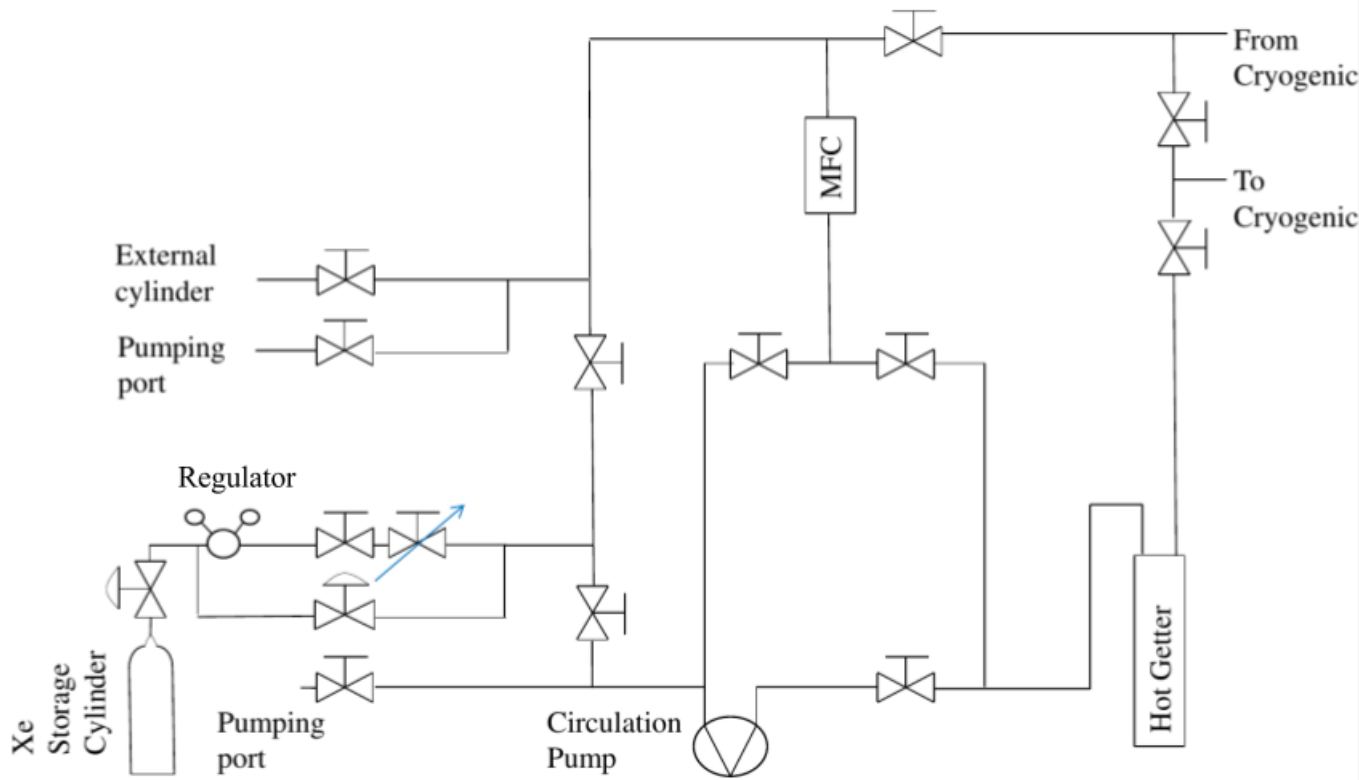
\includegraphics[width=0.75\linewidth]{GasSchematics.png}}
\caption{Schematics of the purification system. High pressure valves are indicated as 
valves with arcs. Needle valves are indicated as 
a valve with an arrow.}
\label{fig:gasSchematic}
\end{figure}
%%%%%%%%%%%%%%%%%%%%%%%%%%%%%%%%%%%%%%%%%%%%%%%%%%%%%%%%%%%%%%%%%%%%%%%%%%%%%%%%%%


\subsection{The cryogenic system}
\label{subsec:cryo}

Remote cooling is generally used in LXe experiments due to reduction in background radiation and acoustic noise from the cooler to the detector, and due to design flexibility. The cryogenic system is connected to the gas handling system on 
one side and to the detector part on the other, and built such that replacing the cryo-cooler type (e.g., to PTR) requires just an adaptation to the top flange.


The cryogenic system is divided to an outer vessel (OV) which holds 
the insulation vacuum, and an inner vessel (IV) which holds the xenon. In addition to the vacuum which prevents heat leakage due to diffusion and convection, the IV is completely covered by multi layer aluminized Myler to prevent heating via radiation.  

%%%%%%%%%%%%%%%%%%%%%%%%%%%%%%%%%%%%%%%%%%%%%%%%%%%%%%%%%%%%%%%
\begin{figure}[h]
\centering
\begin{subfigure}[c]{0.25\textheight}
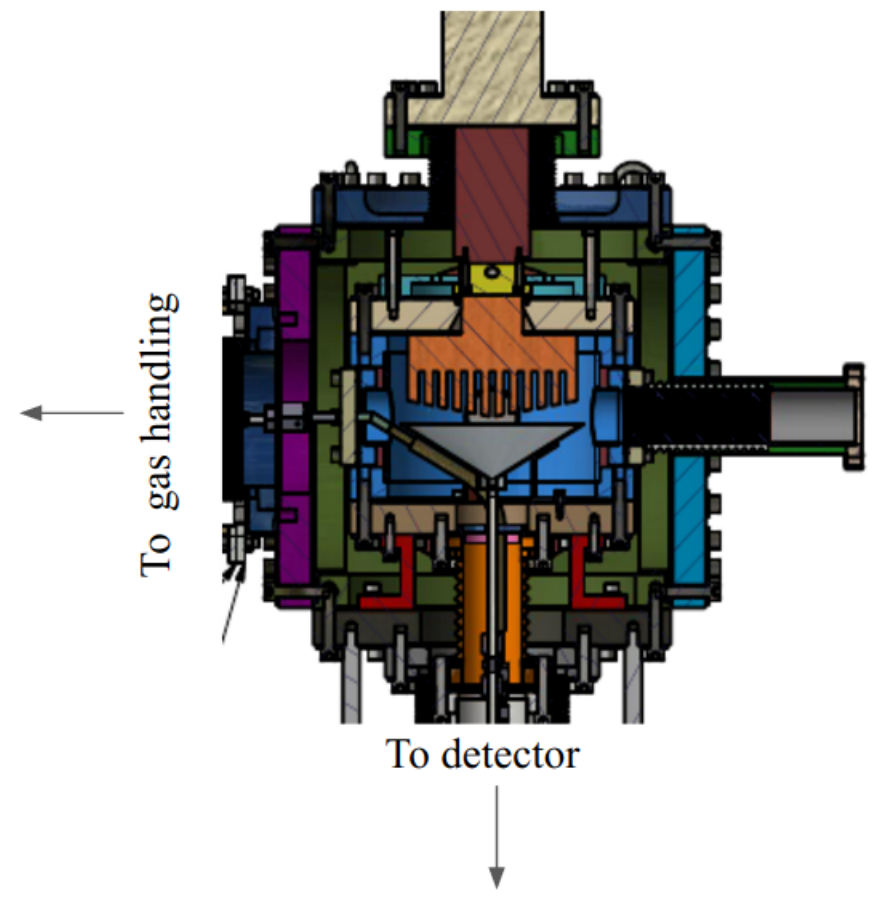
\includegraphics[width=\textwidth]{cryoMirror.png}
\end{subfigure}
\begin{subfigure}[c]{0.25\textheight}
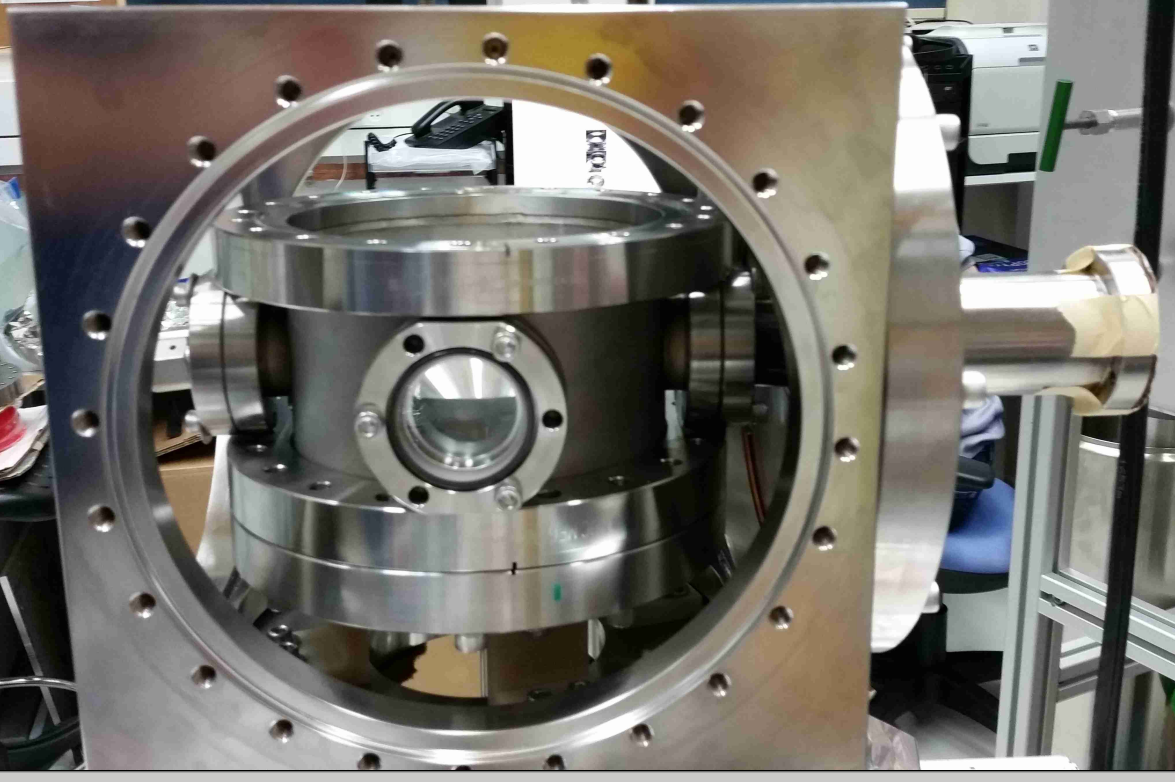
\includegraphics[width=\textwidth]{cryoOpenCrop.png}
\end{subfigure}
\caption{ CAD view of the cryogenic system(Left) and a picture of the cryogenic system (Right) . 
The cryogenic system. (Left) CAD design view, 
(right) picture of the actual system.
\label{fig:cryo}}
\end{figure}
%%%%%%%%%%%%%%%%%%%%%%%%%%%%%%%%%%%%%%%%%%%%%%%%%%%%%%%%%%%%%%%%

The OV is made of a 10" Conflat (CF) cube, with ports on all six faces, interfacing the gas handling system and  the detector part, and bearing service ports (e.g., feed-throughs, pumping ports, 
view ports). The OV is connected to the detector part via a 6" CF flexible bellows, providing a shared vacuum.

The IV is made of 1.5" long cylinder with 6" CF flanges on both sides, holding xenon within. A 120~\,mm diameter cold finger is welded to its top flange. The design of the cold finger is similar to the one in~\cite{xe100_instr2012}. The inner part of the cold finger is made of long fins, resulting in a better heat transport.  The upper part of the cold finger is in thermal contact with the 
QDrive cryo-cooler~\footnote{QDrive 20BB 9p6 A 3 AYNBNCO} via a copper adapter. The copper adapter 
holds two $100\Omega$ pt resistor which are connected to a PID reader\footnote{cryo-con model 
18i Cryogenic Temp Monitor} for temperature measurements. A cartridge-heater 
is also inserted to the copper adapter for emergency heating in case xenon freezes on the 
cold finger. 

The cryo-cooler is connected via a $4\frac{1}{2}$" 
flange to the OV top flange. While usually cryo-coolers used for 
xenon experiments constantly operate in maximal cooling, the QDrive cryo-cooler utilizes a 
temperature control to vary its cooling power up to 70\,W. This allows setting a desired working temperature which is constant within less then $0.1~\mathrm{^{\circ}C}$ measured on the cryo-cooler.

On the inner side of the IV bottom flange a thin 0.6~mm SS funnel is installed 
collecting LXe drops from the cold finger, and delivering them to the  detector part. 
This flange is attached to the detector part, via a $3\frac{3}{8}$" flexible bellows. This 
bellows hosts two pipes connected to the circulation system, and a third pipe coming 
from the funnel. The three pipes deliver LXe whereas the GXe is filling the bellows volume. The purer LXe (from the gas handling system) and the less pure LXe (from the cold finger) are separated, and can be delivered to different parts of the system. Some of the guidelines for the design of 
the cryogenic system are based on~\cite{Giboni}. The CAD view of 
the design of the cryogenic system and a photo of the actual system are shown in Fig~\ref{fig:cryo}. 

%%%%%%%%%%%%%%%%%%%%%%%%%%%%%%%%%%%%%%%%%%%%%%%%%%%%%%%%%%%%%%%%%%%%%%%%%%%%%%%%%%%%%%%%%%%%%%%%%%%%%%%%%%%%%%%%%%%%%%%%%%%%%%%%%%%%%%%%%%%%%%%%%%%%%%%%%%%%%
\subsection{The detector system}
\label{subsec:det}
 
The detector system refers to the chamber and its inner assembly consisting of a transparent sphere that 
contains the LXe, the photomultiplier sensors observing it and their accessories. This chamber is placed below the cryogenic system. 


%mmd{I feel 
%that when we say ``these two parts'', it might not be a clear statement. We may either skip what we describe entirely, 
%or might keep it as in the following.} \RanComment{agreed I think we can drop this , the paper is short enough so we don't need to detail where we describe what.}
%We describe the detector chamber and its interface to the cryogenic system in 
%section \ref{subsubsec:detchamber}. In section \ref{subsubsec:sphere} we discuss the assembly 
%%around the sphere.
%%%%%%%%%%%%%%%%%%%%%%%%%%%%%%%%%%%%%%%%%%%%%%%%%%%%%%%%%%%%%%%%%%%%%%%%%%%%%%%%%%%%%%%%%%%%%%%%%%%%%%%%
%\subsubsection{The Detector Chamber}
%\label{subsubsec:detchamber}

The interface unit to the cryogenic system is built out of 2 flanges welded together via 7 tubes, which serve as service ports for electrical and other feedthroughs, 4 
with a $2 \frac{3}{4}/$ CF flange, and 3 with a $1\frac{1}{3}$ CF flange (mini-CF). 
The upper flange, ISO-K NW320, shares the cryogenic system's OV insulation vacuum, while the bottom one, CF-10", is part of the IV for future detectors, and could hold xenon. 
In addition the CF flange is adapted to fit a smaller CF-$4\frac{5}{8}$" flange which is currently used.

The chamber is made of a ISO-K NW320 nipple closed with a blank flange from below, 
the length of the nipple is determined such that the maximal height of the whole 
apparatus is 190~\,cm, allowing an easy transport of the detector through standard doors.
 
The $4\frac{5}{8}$" CF flange is connected to a split vessel that serves as a LXe reservoir. one part is connected 
to the HPFS sphere from above, and one from below. LXe is circulated such that new LXe drips into the one part and pumped from the other to the gas handling system. This controls the liquid level, and the sphere is constantly filled with LXe. 


The sphere is a custom designed hollow shell made of Corning HPFS 8655 with high transmittance to VUV. Two invar tubes with SS mini-CF flange are connected to the sphere on both sides. The technical design and image of the sphere are shown in Fig.~\ref{fig:sphere}. The optical properties of the sphere will be further discussed in~\ref{sec:opt} 
The bottom flange of the sphere is held using a brass holder to prevent 
force or torque applied on the sphere while mounting it. The 
brass holder is connected to a plate held from the top CF-10" flange. 
%A set of 20 
%PMTs\footnote{R8520-406 Hamamatsu 1" PMT, active area 20.5 mm $\times 20.5 mm$} 
%are placed around the sphere to detect light emitted from the LXe.


%%%%%%%%%%%%%%%%%%%%%%%%%%%%%%%%%%%%%%%%%%%%%%%%%%%%%%%%%%%%%%%%%%%%%%
\begin{figure}[h]
\centering
\begin{subfigure}[c]{0.4\textheight}
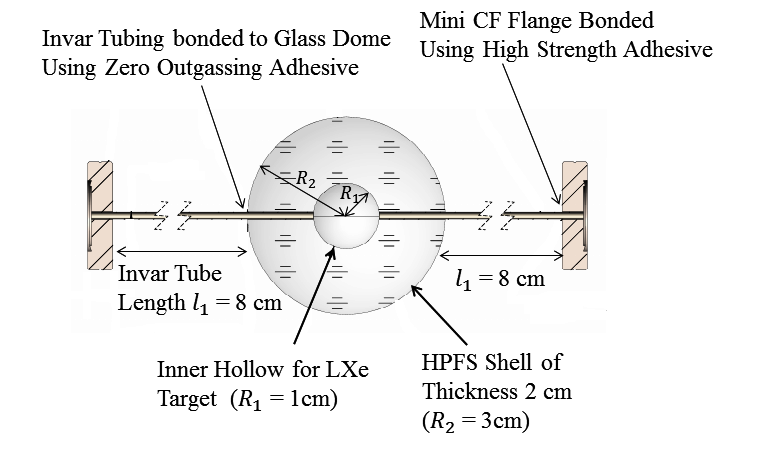
\includegraphics[width=\textwidth]{spheredesign1.png}
\end{subfigure}
\begin{subfigure}[c]{0.25\textheight}
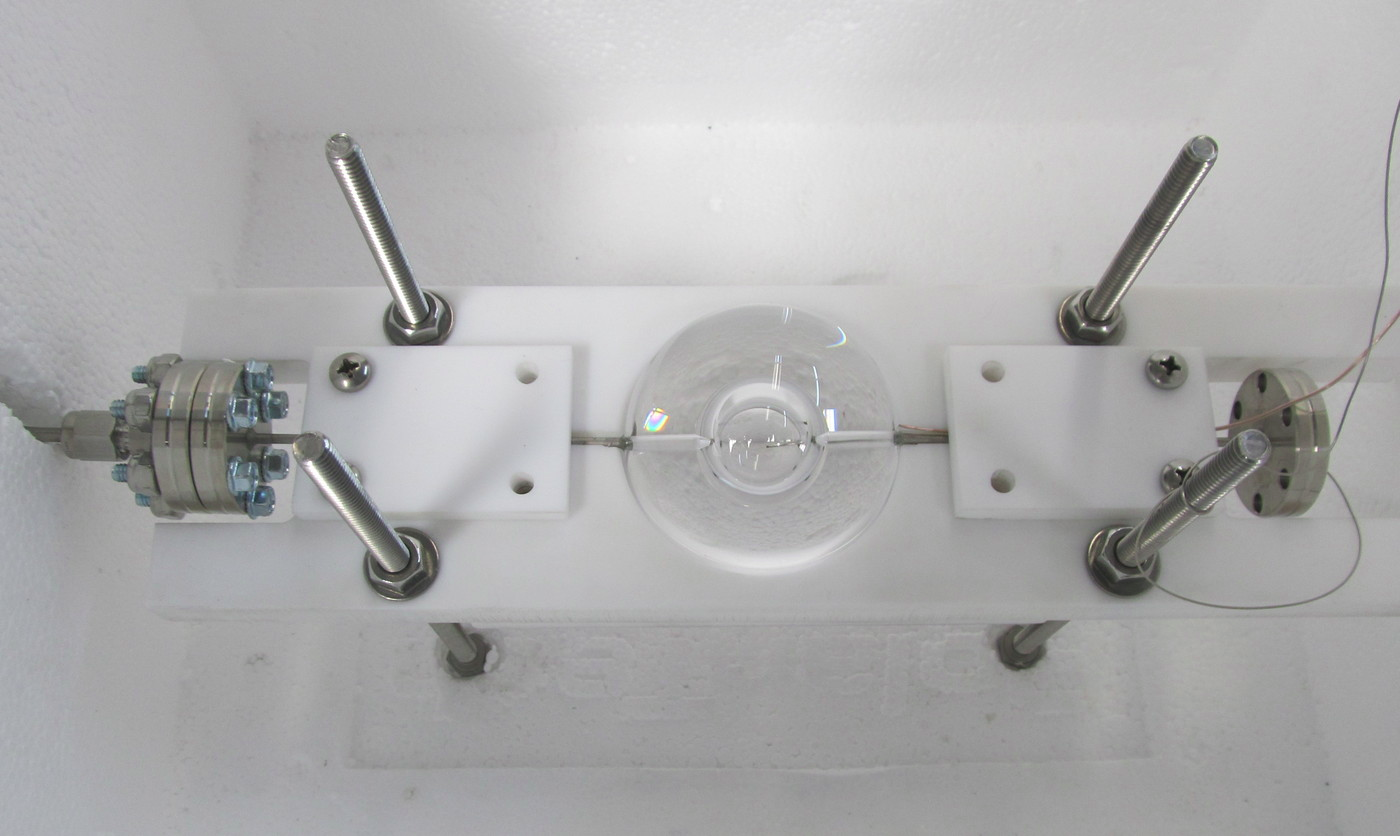
\includegraphics[width=\textwidth]{spherephoto.png}
\end{subfigure}
\caption{(Left)The technical design of the HPFS shell with invar tubing and mini CF flanges. 
(Right) The industrially manufactured HPFS shell.} 
\label{fig:sphere}
\end{figure}
%%%%%%%%%%%%%%%%%%%%%%%%%%%%%%%%%%%%%%%%%%%%%%%%%%%%%%%%%%%%%%%%%%%%%%%%



Photons emitted from the LXe in the sphere are detected by 20  PMTs\footnote{R8520-406 Hamamatsu 1" PMT, active area 20.5 mm $\times 20.5 mm$}. 
The PMTs are chosen to have a quantum efficiency greater than 30\% at 178\,nm. The gain of the PMTs is ~ 2 $\times$ 10$^6$ at an applied voltage of 900\,V . A positive voltage divider, 
manufactured by Hamamatsu, is used to to provide high voltage to the PMTs. 
The PMTs are held with a special aluminum holder, coated with anti-reflection substance. 
The holder is made of two hemispheres hosting the PMTs in 3 rows all of them pointing to the 
center of the sphere. The PMTs are attached to the holder by their voltage--divider bases using M2 PEEK screws see Fig~\ref{fig:pmtholder}. 
The CAD design and a photo of the detector system are shown 
in Fig.~\ref{fig:detector}.

%%%%%%%%%%%%%%%%%%%%%%%%%%%%%%%%%%%%%%%%%%%%%%%%%%%%%%%%%%%%%%%%%%%%%%%%%%%%%%%%%%%%%%%%%%%
\begin{figure}[h]
   \centering
   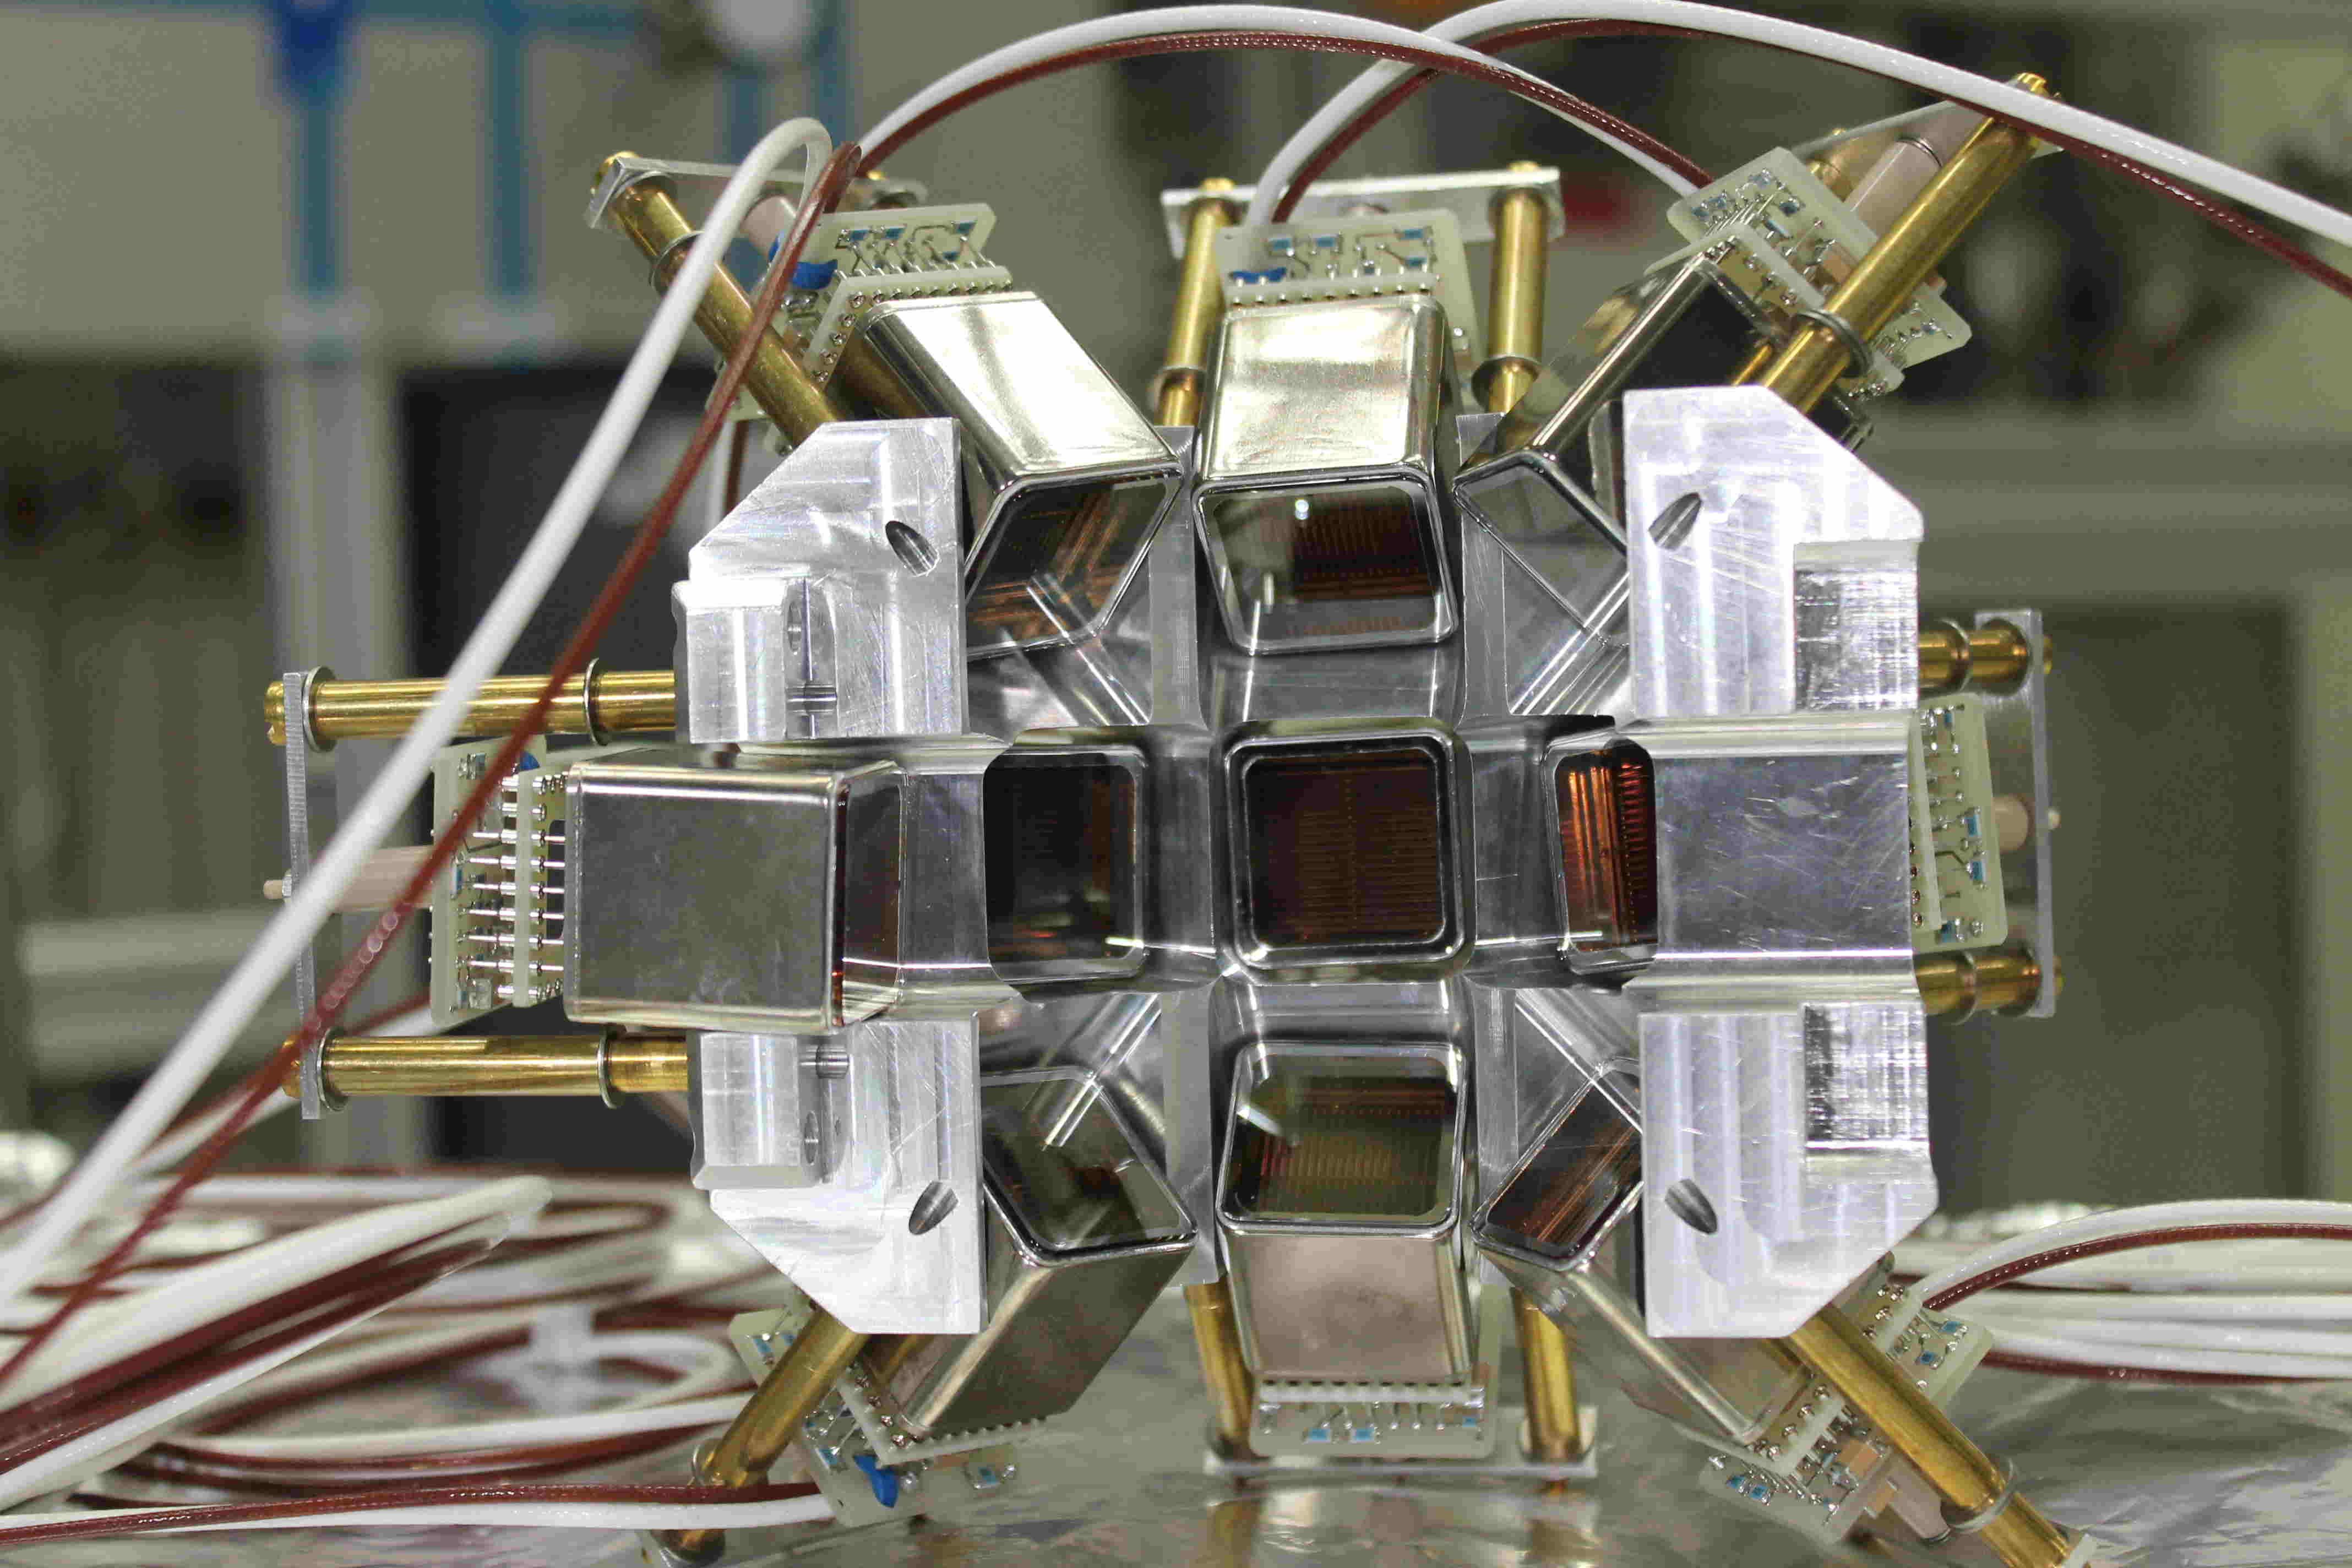
\includegraphics[width=0.5\textwidth]{PMTholder.JPG}
   \caption{A PMT holder--hemisphere. Two identical hemispheres are used to hold the PMTS around the sphere.} 
   \label{fig:pmtholder}
\end{figure}
%%%%%%%%%%%%%%%%%%%%%%%%%%%%%%%%%%%%%%%%%%%%%%%%%%%%%%%%%%%%%%%%%%%%%%%%%%%%%%%%%%%%%%%%%%%

%%%%%%%%%%%%%%%%%%%%%%%%%%%%%%%%%%%%%%%%%%%%%%%%%%%%%%%%%%%%%%%%%%%%%%%%%%
\begin{figure}[h]
\centering
\begin{subfigure}[c]{0.45\textwidth}
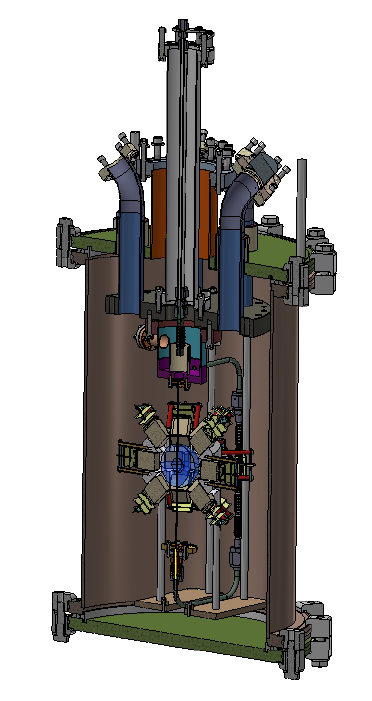
\includegraphics[width=0.75\textwidth , height=0.3\textheight]{detCAD.png}% Here is how to import 
\end{subfigure}	
\begin{subfigure}[c]{0.45\textwidth}
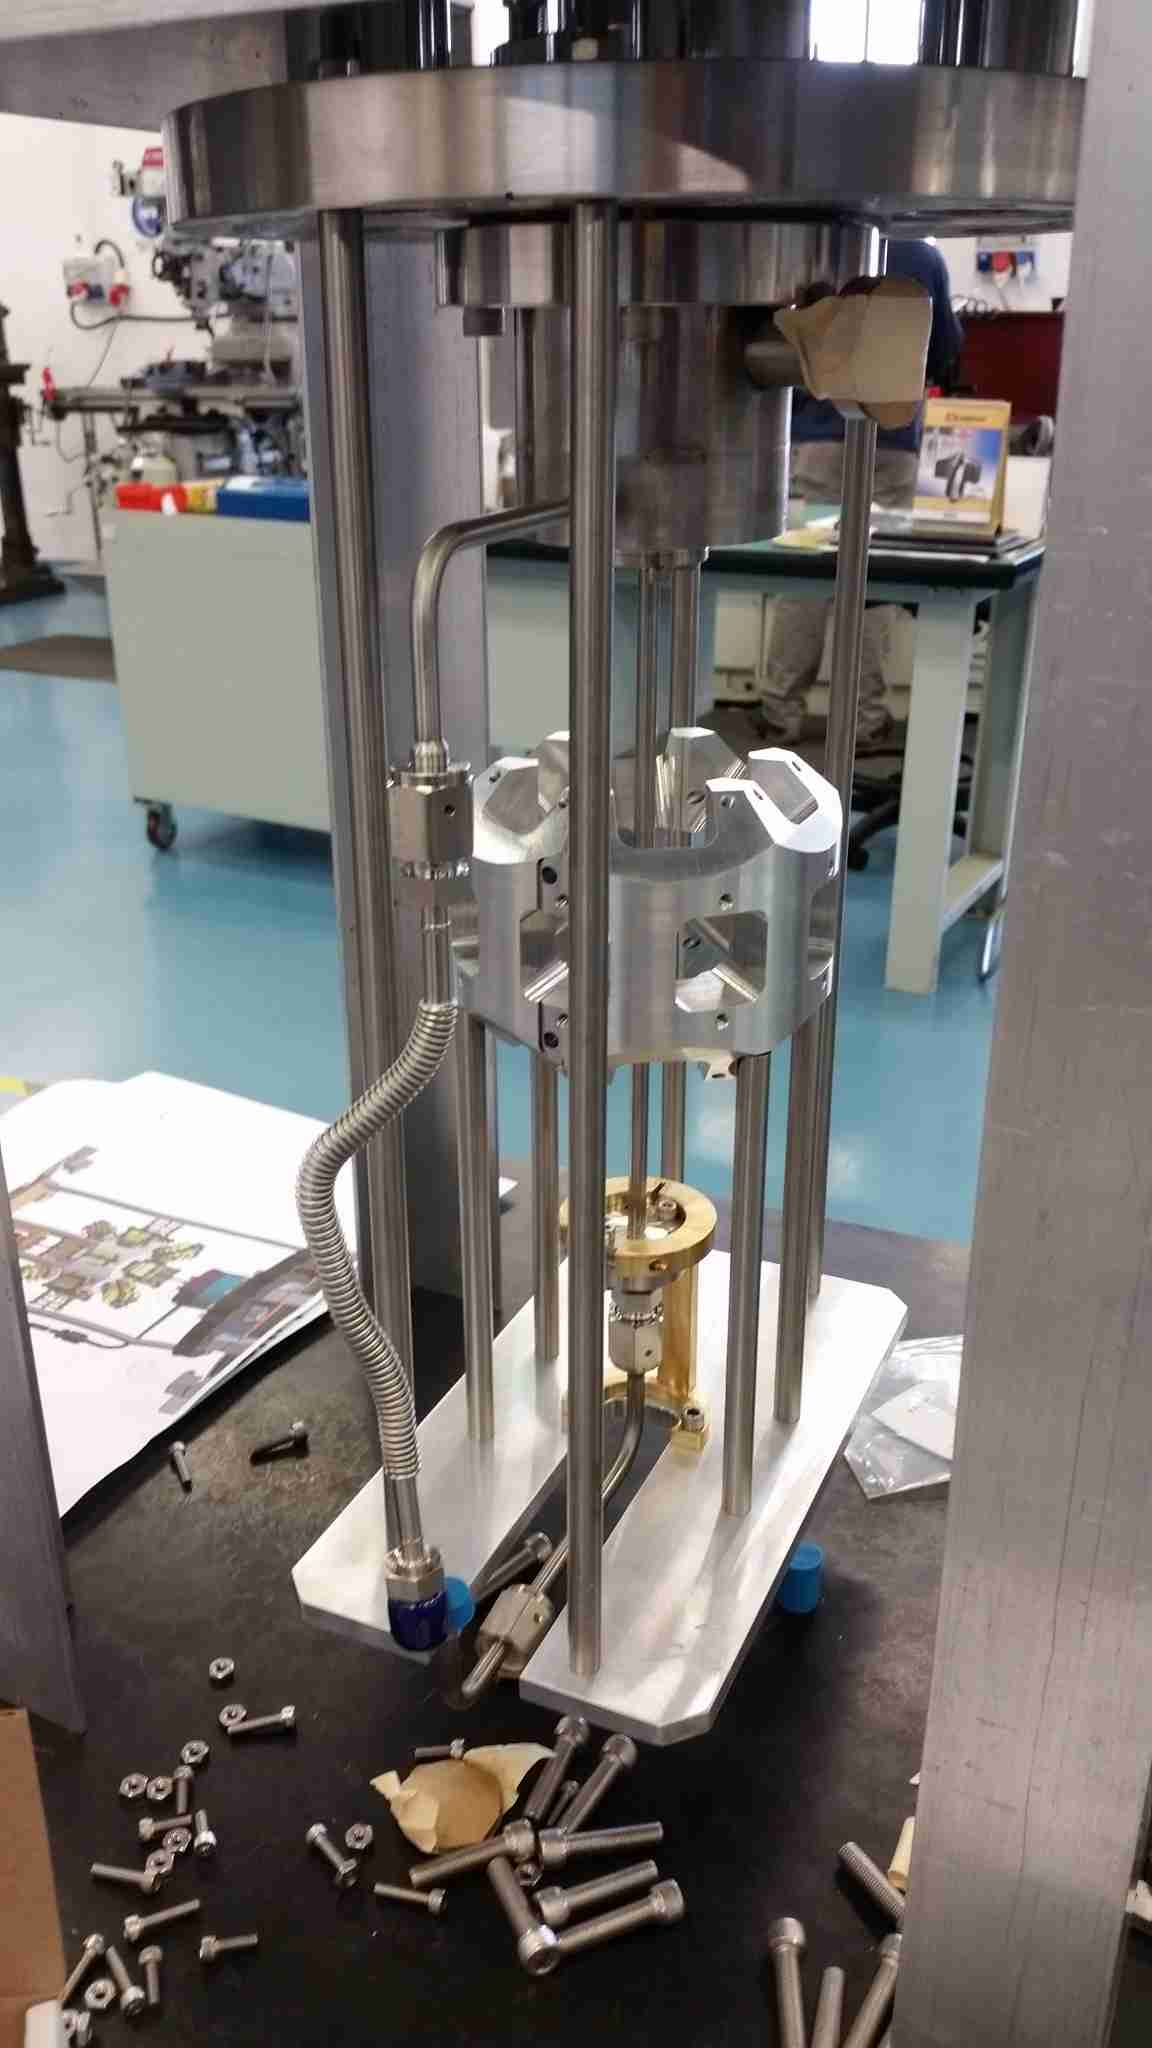
\includegraphics[width=\textwidth , height=0.3\textheight]{detReal_small.jpg}% Here is how to import 
\end{subfigure}	
\caption{\label{fig:detector} (Left) CAD design of the detector part. (Right) First mounting of the 
detector part, still not connected to the rest of the system.}
\end{figure}


%%%%%%%%%%%%%%%%%%%%%%%%%%%%%%%%%%%%%%%%%%%%%%%%%%%%%%%%%%%%%%%%%%%%%%%%%%%%%%%%%%%%%%%%%%%%%%%%%%%%%%%%%%%%%%%%%%%%%%%
%\subsubsection{The Sphere}
%\label{subsubsec:sphere}

%The central component of the detector assembly is a hollow sphere 
%which holds the LXe bubble. A spherical shell made of Corning HPFS 8655 with high transmittance is 
%designed to hold the LXe target. Two invar tubes 
%are connected to the HPFS sphere from the top and bottom with 
%SS mini-CF flanges at the end, which allows circulation of xenon through 
%the sphere. The technical design and image of the sphere are shown in Fig.~\ref{fig:sphere}. 
%The bottom flange of the sphere is held using a brass holder to prevent 
%force or torque applied on the sphere while mounting the detector. The 
%brass holder is connected to a plate held from the top 8" flange, and is 
%also used to align this plate at first installation. A set of 20 
%PMTs\footnote{R8520-406 Hamamatsu 1" PMT, active area 20.5 mm $\times 20.5 mm$} 
%are placed around the sphere to detect light emitted from the LXe.
%
%
%%%%%%%%%%%%%%%%%%%%%%%%%%%%%%%%%%%%%%%%%%%%%%%%%%%%%%%%%%%%%%%%%%%%%%%
%\begin{figure}[h]
%\centering
%\begin{subfigure}[c]{0.4\textheight}
%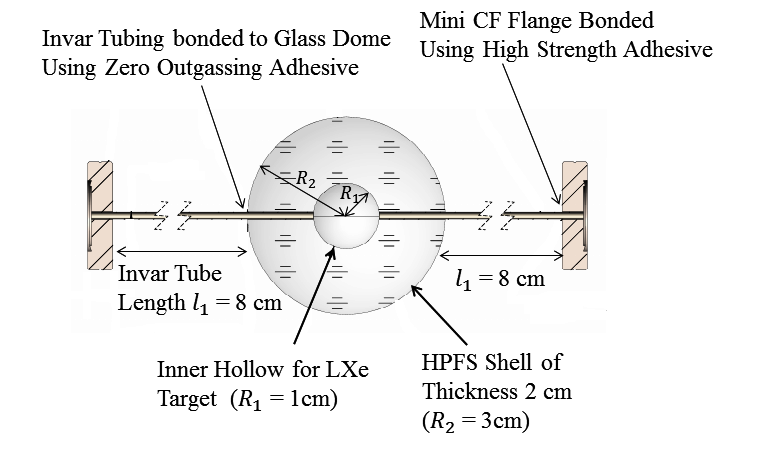
\includegraphics[width=\textwidth]{spheredesign1.png}
%\end{subfigure}
%\begin{subfigure}[c]{0.25\textheight}
%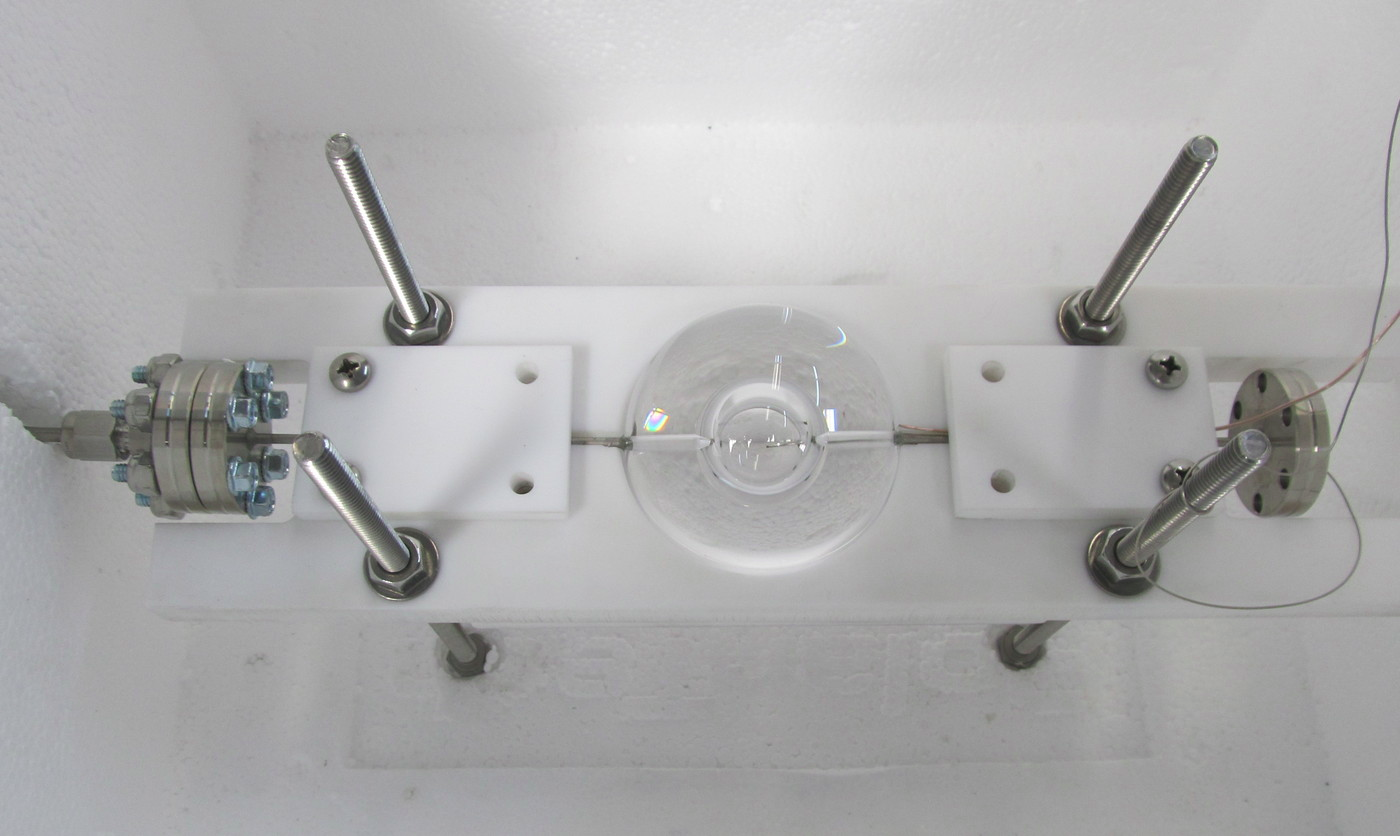
\includegraphics[width=\textwidth]{spherephoto.png}
%\end{subfigure}
%\caption{(Left)The technical design of the HPFS shell with invar tubing and mini CF flanges. 
%(Right) The industrially manufactured HPFS shell.} 
%\label{fig:sphere}
%\end{figure}
%%%%%%%%%%%%%%%%%%%%%%%%%%%%%%%%%%%%%%%%%%%%%%%%%%%%%%%%%%%%%%%%%%%%%%%%%
%


%The LXe target bubble should not be too large in order to avoid double scatters. 
%The HPFS shell should be large enough to reduce internal reflections, but not 
%too large which would attenuate the scintillation light. The material of the 
%shell should have a refractive index as similar to LXe as possible in order to 
%have minimal diffraction from the original direction of the photons when they 
%travel from the LXe target to the sphere. Corning HPFS 8655 is chosen as the shell 
%material. The refractive index of HPFS 8655 is 1.575 at 185 nm (LXe R.I. 1.61). 
%In Fig.~\ref{fig:hpfsRIcalibration} (left panel), are the refractive indexes at various wavelengths 
%as provided on the HPFS 8655 fact sheet as well as a naive extrapolation to lower wavelengths 
%which are relevant to us. 
%
%\begin{figure}[h]
%   \centering
%   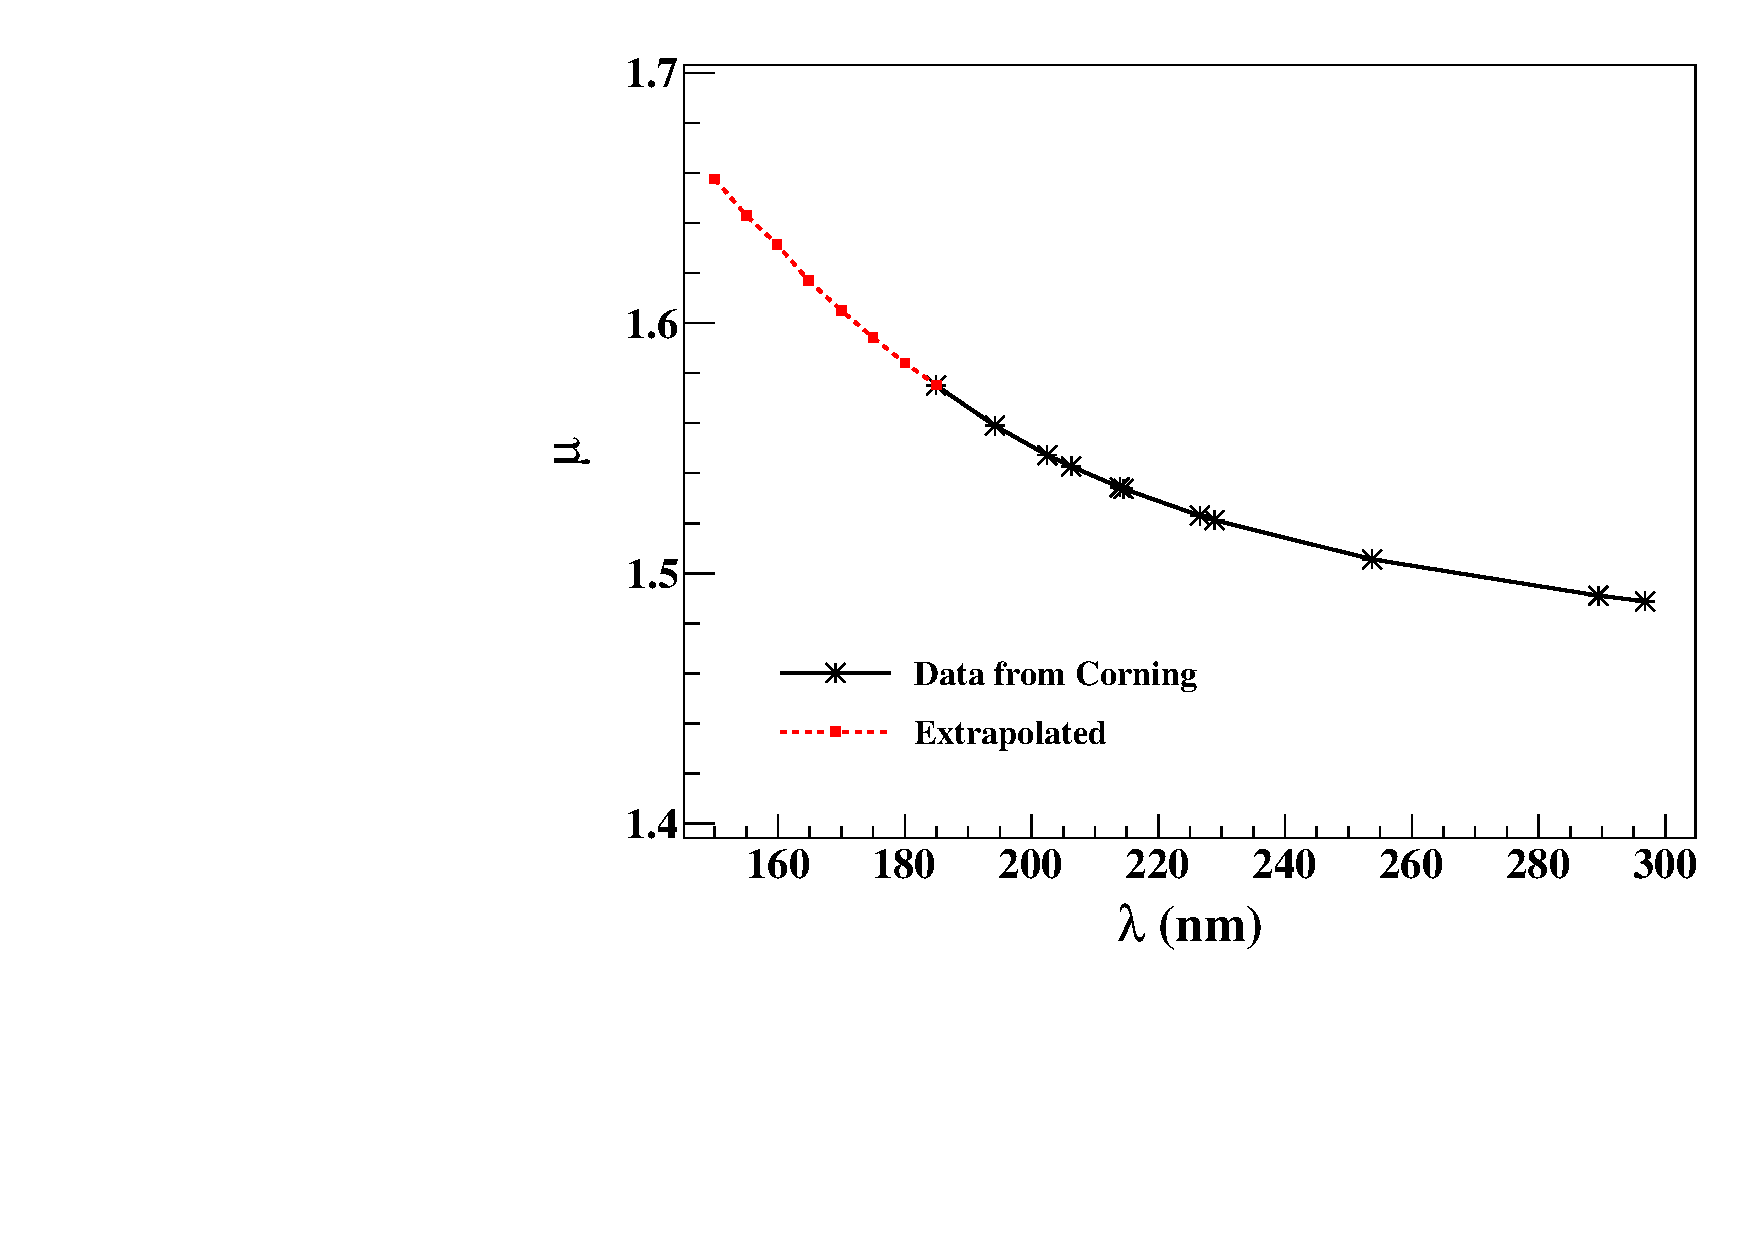
\includegraphics[width=0.48\textwidth]{RI-calibration.pdf}
%    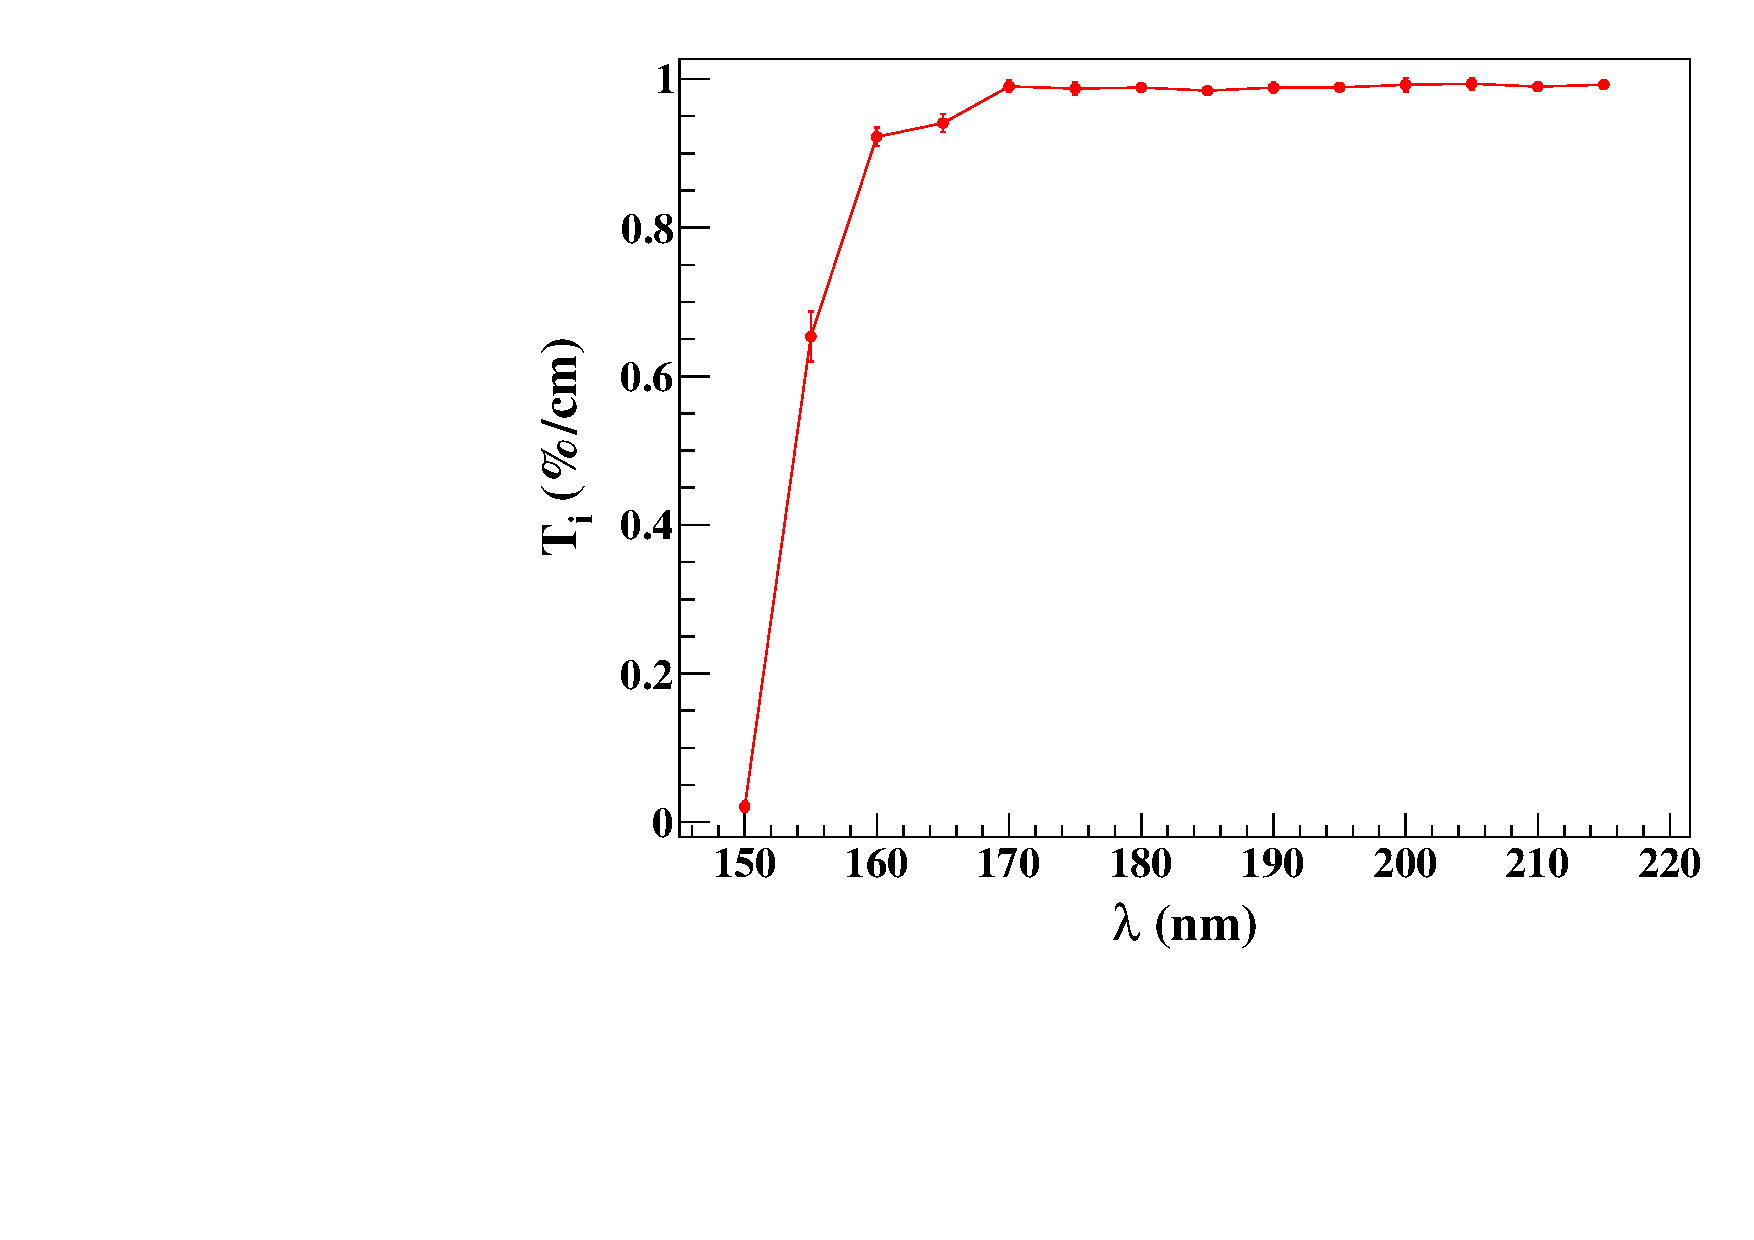
\includegraphics[width=0.48\textwidth]{IntTransmittance.pdf}
%   \caption{The important characteristics of HPFS-8655. (Left) The refractive index as provided by corning and 
%   extrapolated to relevant wavelength range. (Right) The internal transmittance ($T_{i}$).} 
%   \label{fig:hpfsRIcalibration}
%\end{figure}
%
%The transmittance of the material is an extremely crucial parameter to optimize the 
%dimension of the shell. Therefore, a sample of HPFS 8655 was tested for transmittance 
%using a VUV monochromator. 
%In fig.~\ref{fig:hpfsRIcalibration} (right panel), the measured 
%transmittances (\%/cm) at (150 - 215)~\,nm are plotted. At 175~\,nm, the intrinsic transmittance 
%of the sample about 98.7\%/cm.  
%
%
%The dimension of the fused silica shell is optimized by studying the path of the 
%scintillation photons using a GEANT4 based simulation~\cite{AGOSTINELLI2003250}. 
%The sources that will be used for exciting the xenon, and creating the supperradiance 
%(signal) as well as the standard emission (background), will be $^{137} \mathrm{Cs}$ 
%(662 keV) and $^{57} \mathrm{Co}$(122keV \& 136 keV) for ER and $^{241}$AmBe , 
%D-D neutron generator, or neutron produced in an accelerator for NR . The mean 
%free path for this energy is a couple of mm ($^{57} \mathrm{Co}$) and (0.5 - 3) 
%cm ($^{137} Cs$).  The outer radius of the shell is 3 cm, while the inner radius of the 
%hollow space that holds the LXe is 1 cm. 


%Photons coming out of the system are detected by twenty R8520-406 PMTs with an 
%active area of 20.5 mm $\times$ 20.5 mm each. 
%The PMT are chosen to have a minimum 
%quantum efficiency of 30\% at 178 nm. At an applied voltage of 900 
%V the gain of these PMTs is ~ 2 $\times$ 10$^6$. A positive voltage divider, 
%also manufactured by Hamamatsu,  is used to to provide high voltage to the PMTs. 
%The PMTs are held with a special aluminum holder, coated with anti-reflection substance. 
%The holder is made of two hemispheres hosting the PMTs in 3 rows all of them pointing to the 
%center of the HPFS sphere. The PMTs are held only via their voltage--divider bases, while 
%the bases are fixed with M2 PEEK screws. 
%In Fig.~\ref{fig:pmtholder}, one of the holder--hemispheres with the 
%PMTs is shown. A CAD schematic and a real view of the detector assembly are shown 
%in In Fig.~\ref{fig:detector}.
%
%%%%%%%%%%%%%%%%%%%%%%%%%%%%%%%%%%%%%%%%%%%%%%%%%%%%%%%%%%%%%%%%%%%%%%%%%%%%%%%%%%%%%%%%%%%%
%\begin{figure}[h]
%   \centering
%   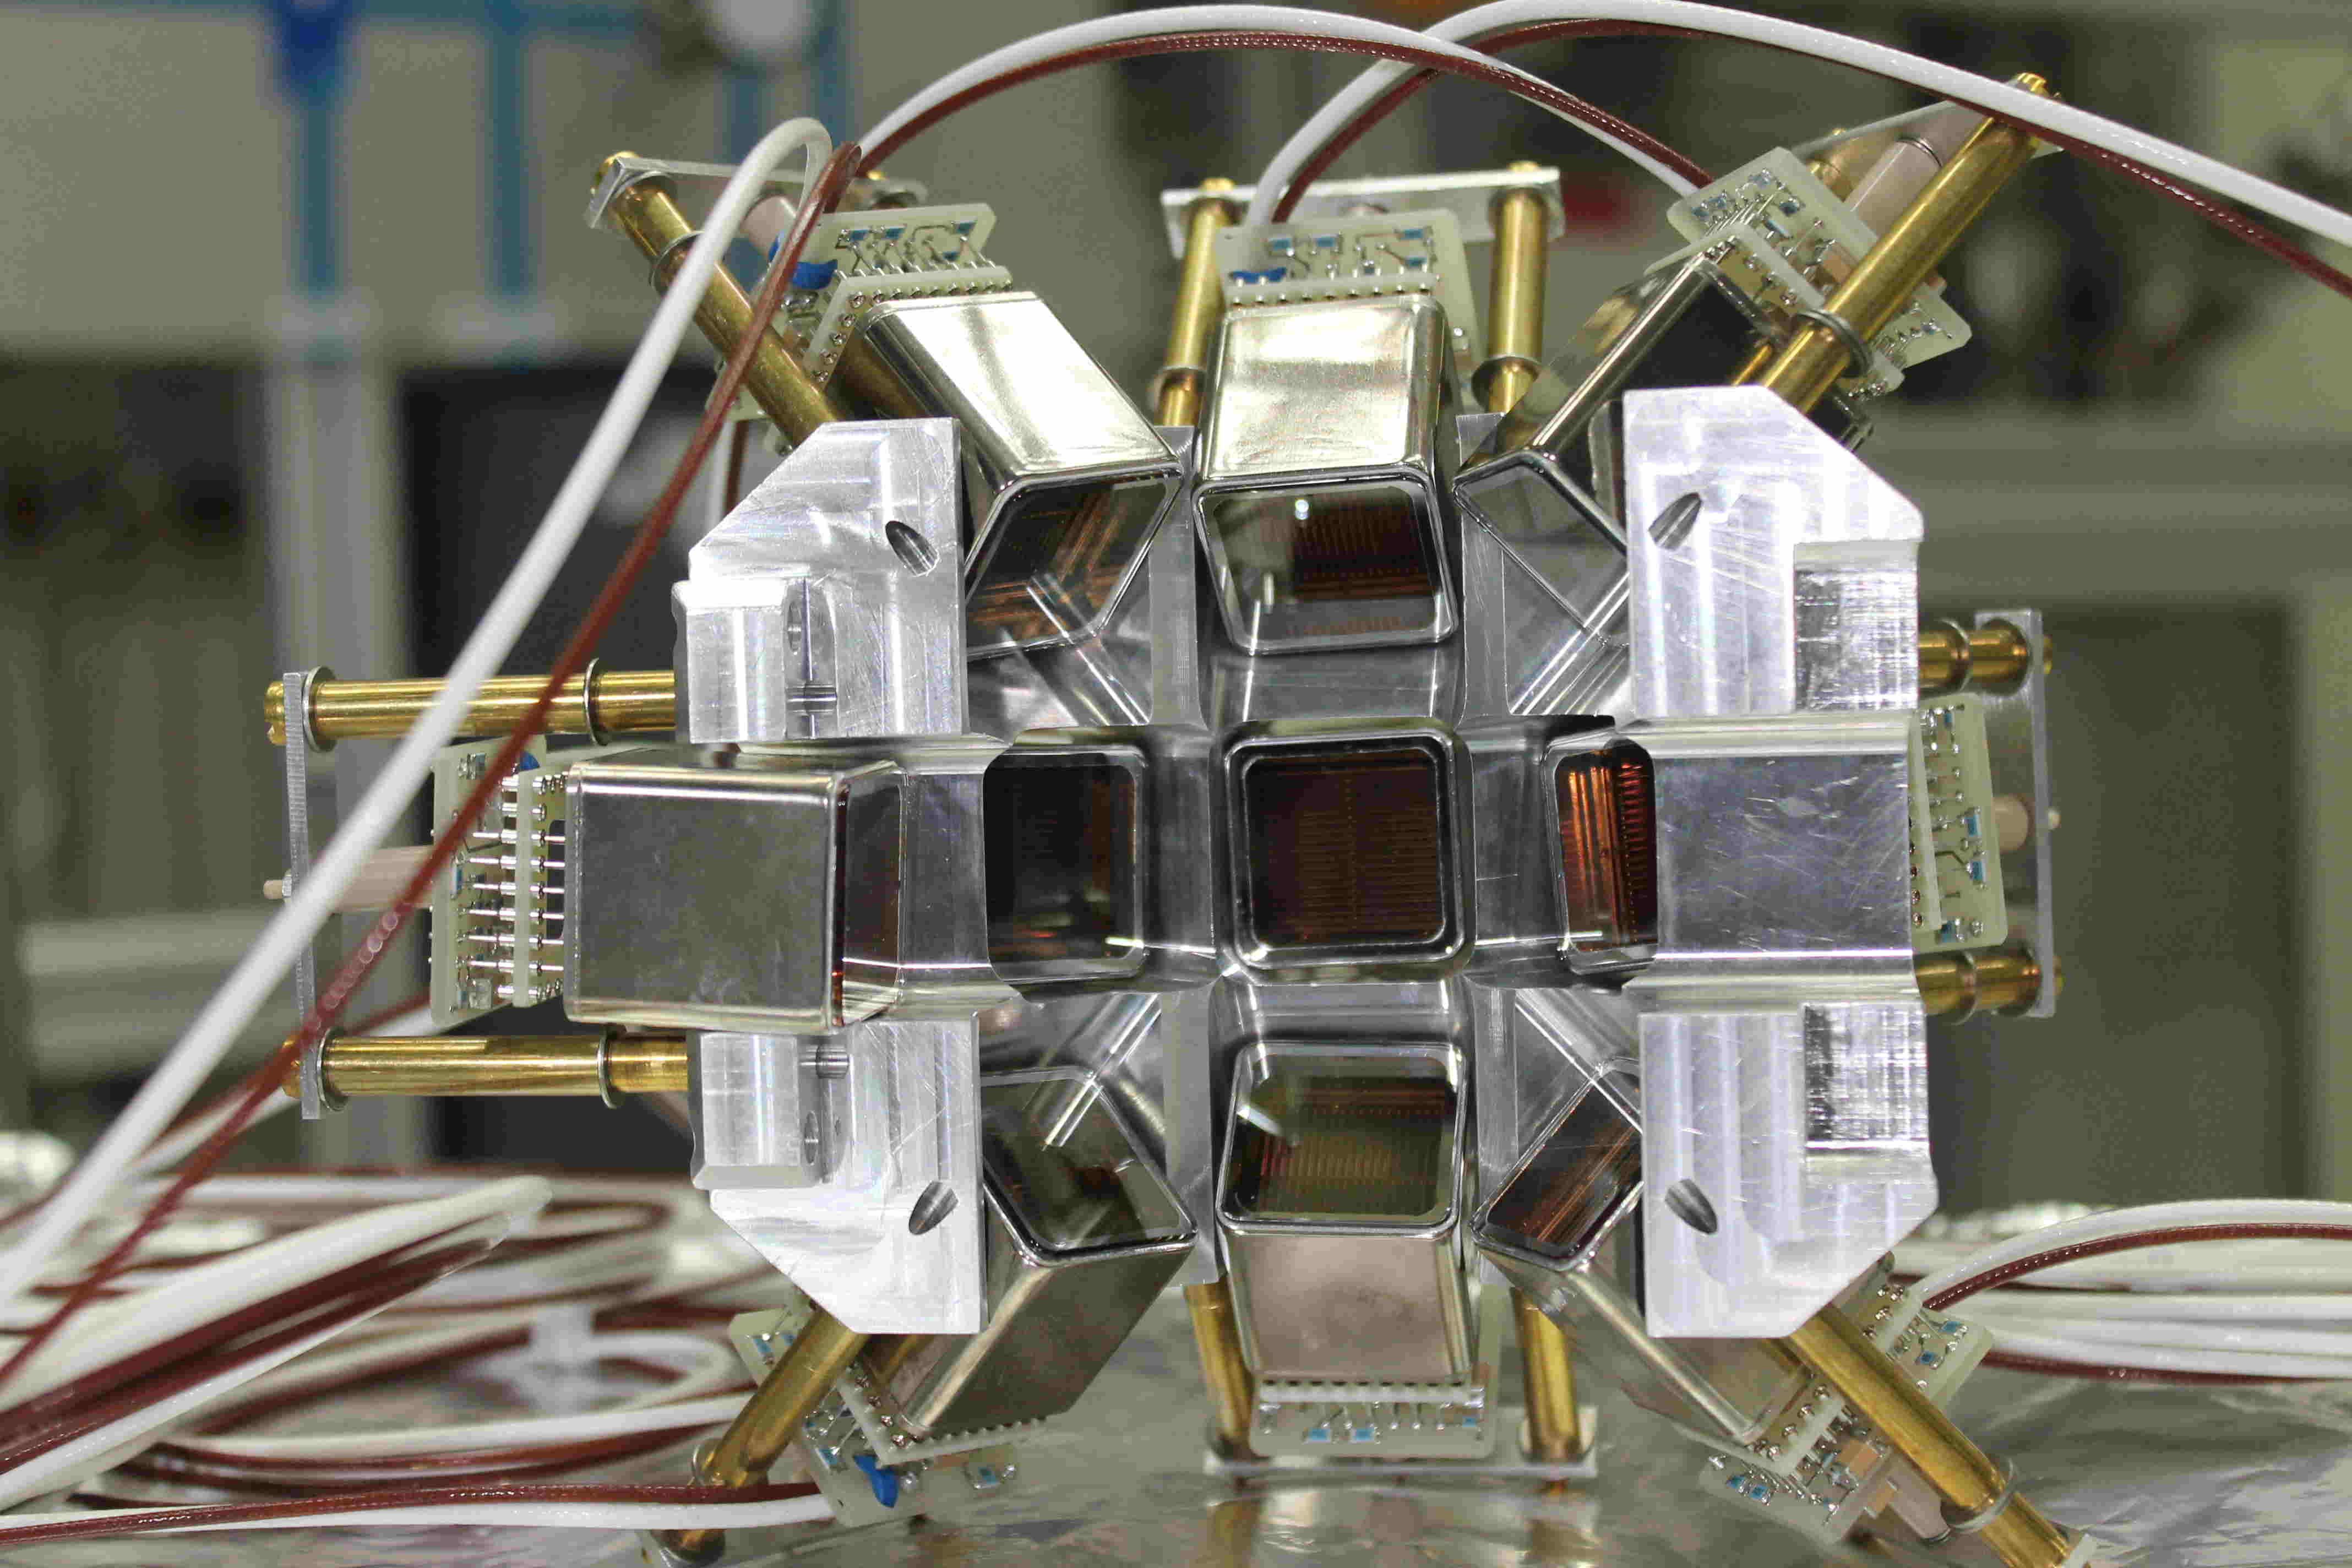
\includegraphics[width=0.5\textwidth]{PMTholder.JPG}
%   \caption{A PMT holder--hemisphere. Two identical hemispheres are used to hold 
%   the PMTS around the HPFS sphere.} 
%   \label{fig:pmtholder}
%\end{figure}
%%%%%%%%%%%%%%%%%%%%%%%%%%%%%%%%%%%%%%%%%%%%%%%%%%%%%%%%%%%%%%%%%%%%%%%%%%%%%%%%%%%%%%%%%%%%
%
%%%%%%%%%%%%%%%%%%%%%%%%%%%%%%%%%%%%%%%%%%%%%%%%%%%%%%%%%%%%%%%%%%%%%%%%%%%
%\begin{figure}[h]
%\centering
%\begin{subfigure}[c]{0.45\textwidth}
%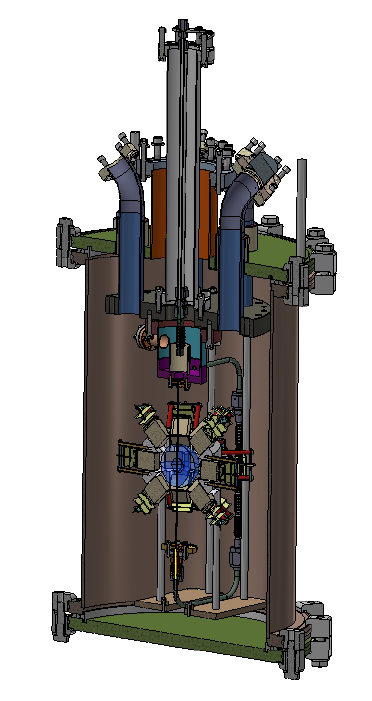
\includegraphics[width=0.75\textwidth , height=0.3\textheight]{detCAD.png}% Here is how to import 
%\end{subfigure}	
%\begin{subfigure}[c]{0.45\textwidth}
%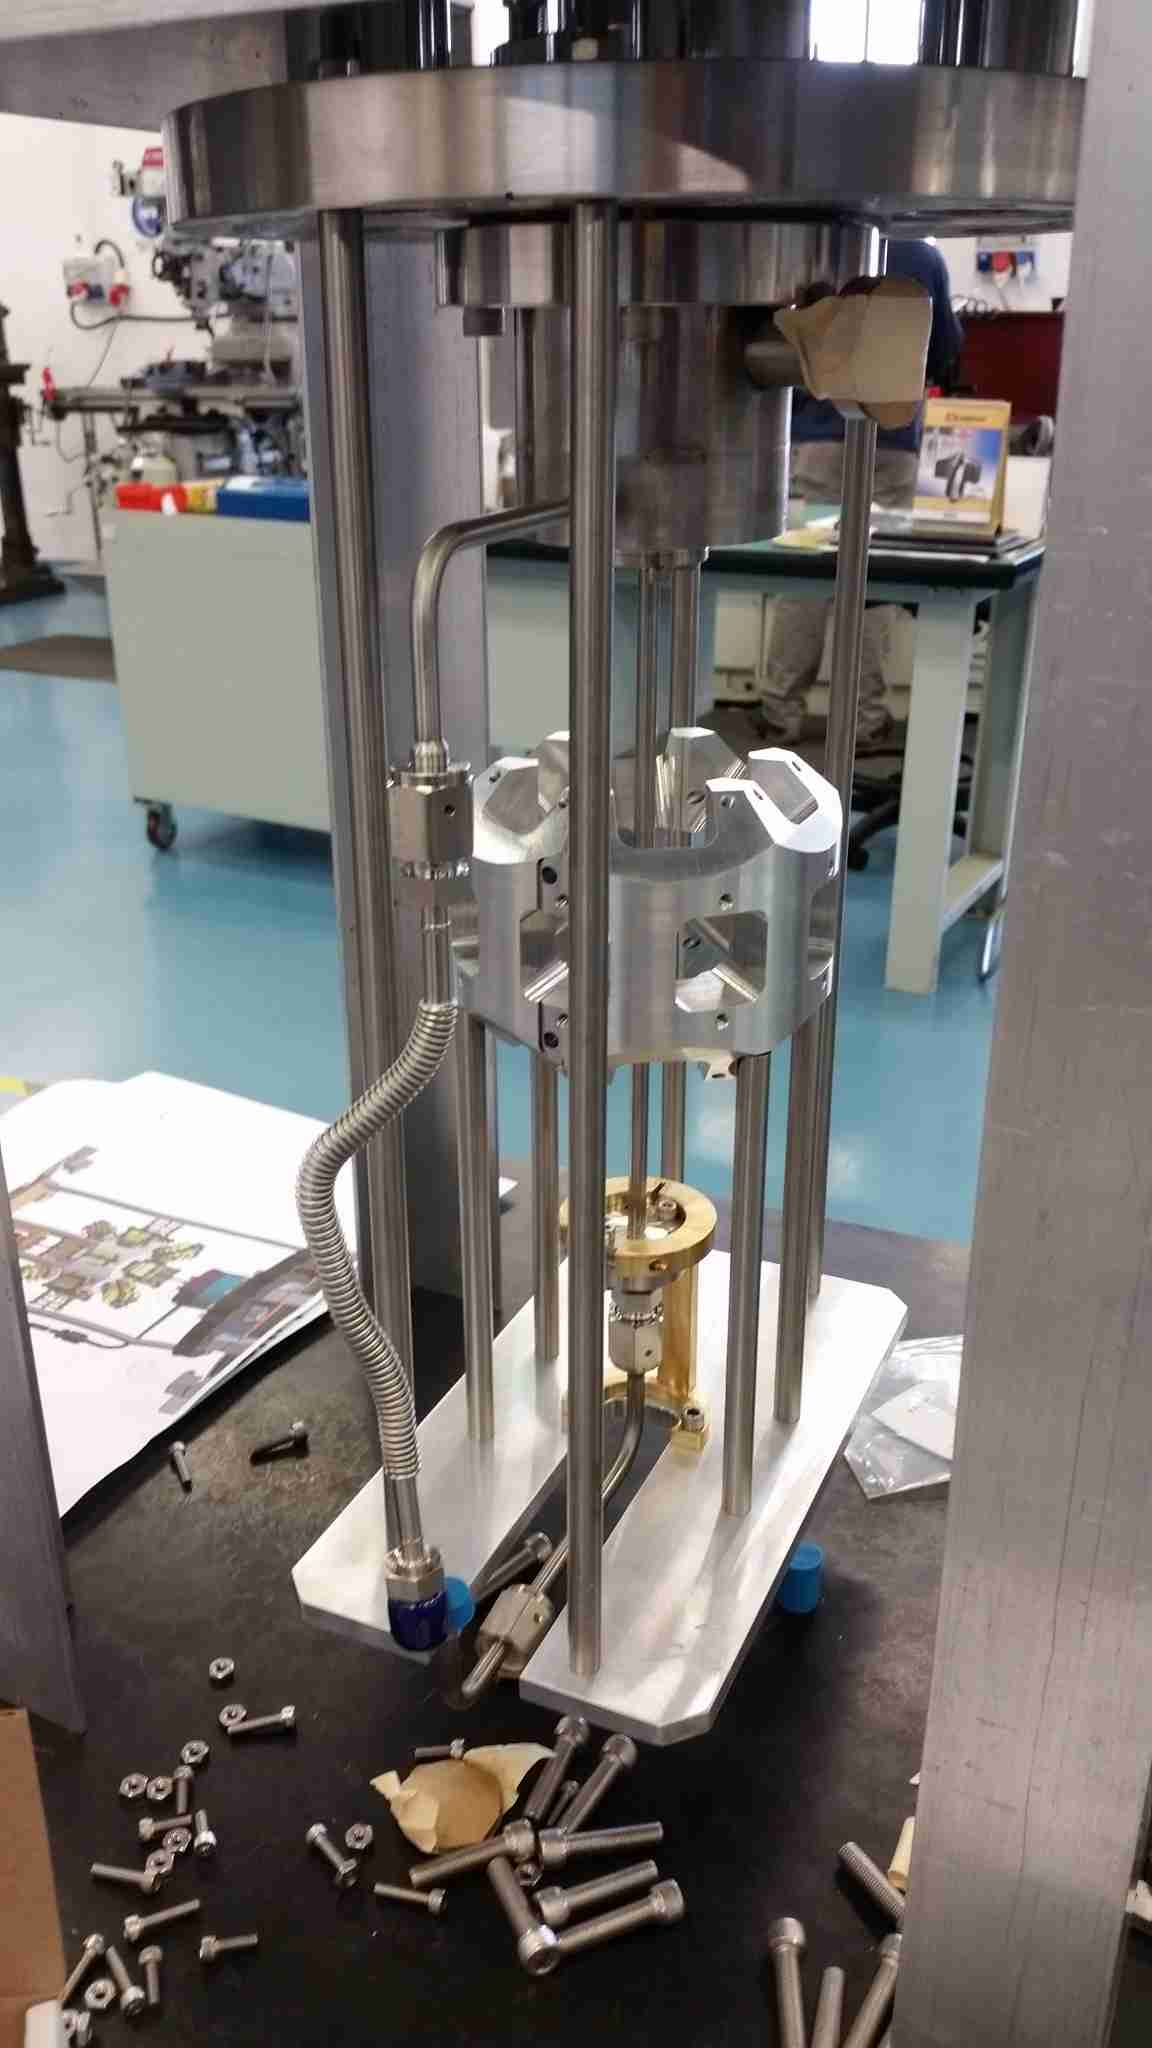
\includegraphics[width=\textwidth , height=0.3\textheight]{detReal_small.jpg}% Here is how to import 
%\end{subfigure}	
%\caption{\label{fig:detector} (Left) CAD design of the detector part. (Right) First mounting of the 
%detector part, still not connected to the rest of the system.}
%\end{figure}
%%%%%%%%%%%%%%%%%%%%%%%%%%%%%%%%%%%%%%%%%%%%%%%%%%%%%%%%%%%%%%%%%%%%%%%%%%%%%
